
\section{Concetti Preliminari}


%\begin{frame}{Web Semantico}
%	Per realizzare il Web Semantico è necessario:
%	\begin{itemize}
%		\item la creazione di formalismi che rappresentino il significato (\textit{\blue{semantica}}) delle informazioni\\$\implies$ \blue{RDF(S)}, \blue{OWL}  - standardizzati da W3C nel 2004
%		\item creare un "Web di dati", invece che di documenti\\$\implies$ IRI, Linked Open Data (LOD) - 2006
%	\end{itemize}
%\end{frame}

\subsection{RDF/OWL}
\begin{frame}{Resource Description Framework (RDF)\footnote{https://www.w3.org/RDF/}}	
	Annotazioni espressive che descrivono dati e le loro relazioni (\textit{\blue{risorse}}). Sono in forma di \blue{triple}:
	\[ ( \textit{soggetto}, \textit{predicato}, \textit{oggetto})\]
	Ogni componente è rappresentata da \blue{IRI}, identificatori deferenziabili che puntano alla vera risorsa (es. \url{http://example.org/\#Pizza}).\\
	Un'insieme di triple rappresenta un \blue{grafo diretto}.

	\begin{center}
		\{(Margherita, \textit{type}, Pizza),\\
		(Vegetarian, \textit{mangia}, Margherita),\}
		\[\equiv\]
		\begin{tikzpicture}[
			node distance = 10mm,
			V/.style = {rounded corners, font=\footnotesize, draw, fill=gray!30},
			every edge quotes/.style = {auto, font=\footnotesize, sloped}
			]
			\begin{scope}[nodes=V]
				\node (1)   {Pizza};
				\node (2) [left=of 1]    {Margherita};
				\node (3) [left=of 2]    {Vegetarian};
			\end{scope}
			\draw[->, ultra thick]   (2)  edge["\textit{type}"] (1)
			(3)  edge["\textit{mangia}"] (2);
		\end{tikzpicture}
		
	\end{center}
	
\end{frame}
\begin{frame}{Ontology Web Language (OWL)\footnote{https://www.w3.org/OWL/}}

	%Un'ontologia OWL permette la descrizione di una realtà d'interesse, ovvero il significato di tutti i termini utili, la loro struttura tassonomica e eventuali asserzioni interessanti sugli individui.
	OWL è un linguaggio \blue{formale} che descrive ontologie, basato sulle \blue{logiche descrittive (DL)}.
		\begin{block}{Ontologia}
		Rappresentazione formale, condivisa ed esplicita di una concettualizzazione.
	\end{block}
%	Un'ontologia OWL permette una descrizione strutturata della realtà d'interesse. 
	Le DL separano la rappresentazione in due parti, dette \textsc{Box}:
	\begin{itemize}
		\item \textsc{\blue{T-Box}}, definisce il vocabolario del dominio (\blue{concetti} e loro caratteristica);\\
		\blue{$\implies$ relazione di subconcept: Studente~$\sqsubseteq$~Persona~$\sqcap\ \exists frequenta.Corso$}
		\item \textsc{\blue{A-Box}}, asserzioni sugli individui, dipendono dalla \textsc{T-Box}.\\
		\blue{$\implies$ asserzioni di:}
			\begin{enumerate}
				\item \blue{concetto: $\textit{Margherita} : \texttt{Pizza}$}
				\item \blue{proprietà: $(\textit{Gianni}, \textit{Margherita}) : mangia$}
			\end{enumerate}
	\end{itemize}
\end{frame}

\begin{frame}{Ontology Web Language (OWL)\footnote[2]{https://www.w3.org/OWL/}}
	Il compito principale delle ontologie OWL è quello di permettere un ragionamento strutturato e \blue{inferire} nuove relazione fra dati.
	
	\begin{example}
		Per l'esempio precedente, un'ontologia OWL permette di:
		\begin{itemize}
			\item definire i concetti di \texttt{Pizza}, \texttt{Vegetariano} e \texttt{Pizza Vegetariana};
			\item imporre che $\texttt{Pizza Vegetariana} \sqsubseteq \texttt{Pizza}$;
			\item imporre che un $\texttt{Pizza Vegetariana} \sqsubseteq \exists \textit{mangia}.\texttt{Vegetariano}$;
			\item dichiarare che $\textit{Margherita} : \texttt{Pizza}$;
			\item dichiarare che $\textit{Gianni} : \texttt{Vegetariano}$;
			\item dichiarare che $(\textit{Gianni}, \textit{Margherita}) : \textit{mangia}$.
		\end{itemize}
	\end{example}
	Possiamo \blue{inferire} che $\textit{Margherita} : \texttt{Pizza Vegetariana}$.
\end{frame}

\subsection{Linguaggi Funzionali} % Emanuele o Andrea
\begin{frame}[containsverbatim]{Linguaggi Funzionali}
I linguaggi funzionali sono facili da {\color{blue} leggere}, {\color{blue} debuggare} e {\color{blue} dimostrarne la correttezza}.
\begin{columns}[T]

\begin{column}[T]{.4\textwidth}
\begin{center}
Haskell
\end{center} 
\begin{minted}{haskell}
fact :: Int -> Int 
fact 0 = 1
fact n = n * fact (n-1)
\end{minted}
    
\end{column}

\begin{column}[T]{.45\textwidth}
\begin{center}
Java
\end{center} 
\begin{minted}{java}
public int fact(int n){
    int fact = 1;
    for(i = 1; i <= n; i++){
        fact = fact * i;
    }
    return  fact;
}
\end{minted}
    
\end{column}

\end{columns}

\end{frame}

\begin{frame}[containsverbatim]{Linguaggi Funzionali}
I {\color{blue} Data Type} permettono di creare nuovi tipi per descrivere i dati utilizzati in un programma. \\

\begin{block}{data type per un albero binario di interi}
\begin{minted}{haskell}
data Tree = Node Int Tree Tree 
          | Leaf Int
\end{minted}
\end{block}
\begin{example}
\begin{columns}

\begin{column}{.5\textwidth}	
\begin{minted}{haskell}
tree :: Tree	
tree = Node 1 (Leaf 2) (Leaf 3)
\end{minted}
\end{column}	

\begin{column}{.2\textwidth}	
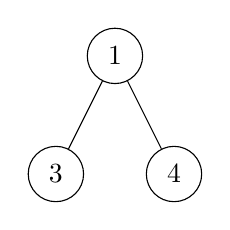
\begin{tikzpicture}[
	every node/.style = {minimum width = 2em, draw, circle},
	]
	\node {1}
	child {node {3}}
	child {node {4}};
  \end{tikzpicture}
\end{column}	

\end{columns}
\end{example}
    
\end{frame}

\begin{frame}[containsverbatim]{Linguaggi Funzionali}
Il {\color{blue} pattern matching} permette di confrontare un argomento con dei pattern per decidere i flusso di esecuzione del programma.\\~\\

\begin{block}{\small Applicazione di fact ad ogni nodo dell'albero}
\begin{minted}{haskell}
mapF :: Tree -> Tree 
mapF (Leaf n)       = Leaf (fact n)
mapF (Node n t1 t2) = Node (fact n) (mapF t1) (mapF t2)
\end{minted}
\end{block}
~\\
\begin{columns}

\begin{column}{0.4\textwidth}	
\centering
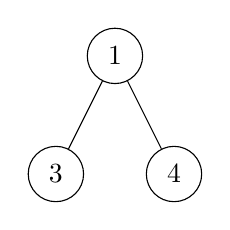
\begin{tikzpicture}[
	every node/.style = {minimum width = 2em, draw, circle},
	]
	\node {1}
	child {node {3}}
	child {node {4}};
  \end{tikzpicture}
\end{column}	
\begin{column}{0.2\textwidth}	
	\LARGE $${\xrightarrow{\textcolor{blue}{mapF}}}$$
\end{column}	
\begin{column}{0.4\textwidth}	
\centering
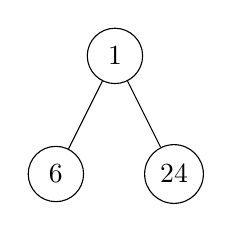
\begin{tikzpicture}[
	every node/.style = {minimum width = 2em, draw, circle},
	]
	\node {1}
	child {node {6}}
	child {node {24}};
  \end{tikzpicture}
\end{column}	

\end{columns}
    
\end{frame}

\begin{frame}[containsverbatim]{Linguaggi Funzionali}
Una {\color{blue} funzione di ordine superiore} pu\`o prendere altre funzioni come argomento e restiturie funzioni come risultato. \\~\\

\begin{block}{\small Applicazione di una funzione passata per argomento ad ogni nodo dell'albero}
\begin{minted}{haskell}
mapT :: (Int -> Int) -> Tree -> Tree 
mapT f (Leaf n)       = Leaf (f n)
mapT f (Node n t1 t2) = Node (f n) (mapT f t1) (mapT f t2)
\end{minted}
\end{block}
~\\
\begin{columns}

\begin{column}{0.2\textwidth}	
\centering
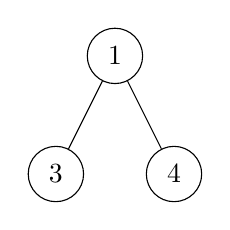
\begin{tikzpicture}[
	every node/.style = {minimum width = 2em, draw, circle},
	]
	\node {1}
	child {node {3}}
	child {node {4}};
  \end{tikzpicture}
\end{column}

\begin{column}{0.2\textwidth}	
\centering
	\Large $${\xrightarrow{\textcolor{blue}{mapT \: fact}}}$$
\end{column}

\begin{column}{0.2\textwidth}	
\centering
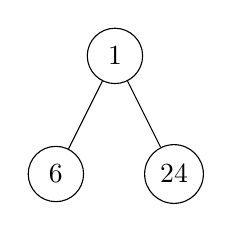
\begin{tikzpicture}[
	every node/.style = {minimum width = 2em, draw, circle},
	]
	\node {1}
	child {node {6}}
	child {node {24}};
  \end{tikzpicture}
\end{column}	

\begin{column}{0.2\textwidth}	
\centering
	\Large $${\xrightarrow{\textcolor{blue}{mapT \: (+1)}}}$$
\end{column}

\begin{column}{0.2\textwidth}	
\centering
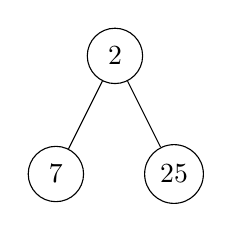
\begin{tikzpicture}[
	every node/.style = {minimum width = 2em, draw, circle},
	]
	\node {2}
	child {node {7}}
	child {node {25}};
  \end{tikzpicture}
\end{column}	

\end{columns}
    
\end{frame}
\subsection{Sistemi di Tipi} % Andrea
\begin{frame}[containsverbatim]{Sistemi di Tipi}
\begin{block}{Type System}
    Un sistema di tipi \`e un metodo sintattico e trattabile per provare l'assenza di alcuni comportamenti del programma classificando i termini in accordo con il tipo
    di valori che computano
\end{block}
\begin{example}
\begin{minted}{java}
 public static void main(String[] args){
	int n = fact(2.2); //errore di tipo
	System.out.println(n);
 }
\end{minted}
\end{example}
\end{frame}

\begin{frame}[containsverbatim]{Sistemi di Tipi}
I sistemi di tipi possono essere usati per dimostrare altre \blue{proprietà} come ad esempio la \blue{correttezza} di una \blue{dimostrazione}.
\begin{block}{Dimostrazione dell'associativit\`a della moltiplicazione (Agda)}
\begin{minted}[escapeinside=||,mathescape=true, fontsize=\small]{agda}
*-assoc : |$\forall$|(x y z : |$\mathbb{N}$|) -> x * (y * z) == (x * y) * z
*-assoc zero y z = refl
*-assoc (succ x) y z =
  begin
	succ x * (y * z)    ==⟨ refl ⟩
	y * z + x * (y * z) ==⟨ cong (y * z +_) (*-assoc x y z) ⟩
	y * z + (x * y) * z   ⟨ *-dist-r y (x * y) z ⟩==
	(y + x * y) * z     ==⟨ refl ⟩
	(succ x * y) * z
  end
\end{minted}
\end{block}
\end{frame}
\begin{frame}[containsverbatim]{Sistemi di Tipi}
\blue{\LARGE Come possiamo usare i linguaggi funzionali e i tipi per le ontologie?}
\end{frame}